\chapter{Hazard and risk results}
\label{ch:risk}


\section{Overview}

Earlier chapters have described how to generate synthetic
earthquakes, propagate (or attenuate) the response spectral
acceleration\index{response spectral acceleration} and compute
loss. This chapter describes how to `aggregate' the above
information to estimate earthquake hazard and earthquake risk. A
number of diagrams are used to demonstrate the common techniques
for visualising earthquake hazard and risk.

\section{Calculating hazard and risk}

Consider a random variable $Y$ such that; \begin{itemize} 

\item
$Y$ refers to the response spectral acceleration\index{response
spectral acceleration} $S_a$ at a particular site in the case of
hazard, or 
\item $Y$ indicates the loss, either at a particular site or
  aggregated building site.  For simplicity we will assume that $Y$
  represents the aggregated loss as a percentage of building stock
  value.
\end{itemize}

A common way to represent $Y$ is in terms of a probability of
exceedance in one year. To achieve this we assume that
earthquakes occur as a Poisson process \citep{dr_McGuire90a}. This
means that the earthquake process has no memory; or in other
words, the probability of an earthquake today does not depend on
whether or not an earthquake occurred yesterday. Mathematically,
this assumption can be represented as follows:
\begin{equation}
 \Pr(T, Y\ge y) = 1 - e^{-\lambda_Y(y)t},
\end{equation}
where t is a time interval in years (typically 1 year) and
$\lambda_Y(y)$ is the annual exceedance rate. The return period is
given by \eref{eq:risk-rptolambda}:
\begin{equation}
\label{eq:risk-rptolambda} R_Y(y) = \frac{1}{\lambda_Y(y)}.
\end{equation}

\subsection{Computing the annual exceedance rate}
\label{sec:risk-ann-exceed-rate}

\cref{ch:source} described the Monte-Carlo approach used to
generate earthquakes. \crefmulti{ch:atten}{ch:losses} describe how
to compute an $S_a$ or loss value for each of the synthetic
events. It follows, therefore that there exists a set of $N_s$
numbers $\{Y_i\}_{i=1}^{N_s}$ with corresponding event activities
$\{r_{\nu _i}\}_{i=1}^{N_s}$ (see \sref{sec:magnitude_selection}),
where $N_s$ is the number of simulated events\index{simulated
event}.

The annual exceedance rate $\lambda_Y(y)$ is computed from the
event activity through the following process:
\begin{enumerate}
\item re-order the values $\{Y_i\}_{i=1}^n$ from largest to
smallest and re-order the corresponding event activities such that
the $Y_i-r_{\nu _i}$ pairs are not separated.
\begin{equation}
\label{eq:eva-vectors1} \left[\begin{matrix}
  y_{1}\\ y_{2} \\ \vdots\\ y_{n}
\end{matrix}\right],
\ \left[\begin{matrix}
 r_{\nu_1} \\ r_{\nu_2} \\ \vdots\\ r_{\nu_n}
\end{matrix}\right]
\to \left[\begin{matrix}
  y_{1^*}\\ y_{2^*} \\ \vdots\\ y_{n^*}
\end{matrix}\right],
\ \left[\begin{matrix}
 r_{\nu_1^*} \\ r_{\nu_2^*} \\ \vdots\\ r_{\nu_n^*}
\end{matrix}\right]
\end{equation}
\item evaluate $\lambda_Y(y)$ by computing the cumulative sum of
event activities.
\begin{equation}
\label{eq:eva-vectors2} \left[\begin{matrix}
 \lambda_{Y_{1^*}}\\ \lambda_{Y_{2^*}} \\ \vdots\\ \lambda_{Y_{n^*}}
\end{matrix}\right] =
\left[\begin{matrix}
  r_{\nu_1^*}\\
   r_{\nu_1^*}+ r_{\nu_2^*} \\
   \vdots\\
   r_{\nu_1^*}+ r_{\nu_2^*} + \ldots + r_{\nu_n^*}\\
\end{matrix}\right],
\end{equation}
\end{enumerate}
The asterisk in \ereftwo{eq:eva-vectors1}{eq:eva-vectors2} refer
to re-ordered values.


\section{Earthquake hazard results}
\label{sec:risk-hzd-results} The EQRM estimates the earthquake
hazard $E_H(R_Y)$ at the return periods $R_Y$ defined in the
EQRM control file by    
interpolating the values $\{ \lambda_{Y_i^*}\}_{i=1}^{N_s}$ and
$\{Y_i^*\}_{i=1}^{N_s}$ to the values $1/R_Y$ (see
\eref{eq:risk-rptolambda}). In the case of earthquake hazard the
random variable $Y$ refers to the response spectral
acceleration\index{response spectral acceleration} and is
therefore a function of building period $T_o$. The earthquake
hazard information is saved in output files. It is important to
emphasise that only the hazard information is saved, the
information for individual synthetic earthquakes is discarded.
This means that the earthquake hazard information can not be
de-aggregated in terms of causative events.

The EQRM offers two tools for visualising the earthquake hazard:
\begin{enumerate}
\item the earthquake hazard map and \item the hazard exceedance
curve.
\end{enumerate}

\subsection{Hazard maps}

Earthquake hazard maps can be used to illustrate the earthquake
hazard across a spatial region. The earthquake hazard $E_H(R_Y)$
is plotted for a specific building period $T_o$ and return period
$R_Y$.
\begin{figure}
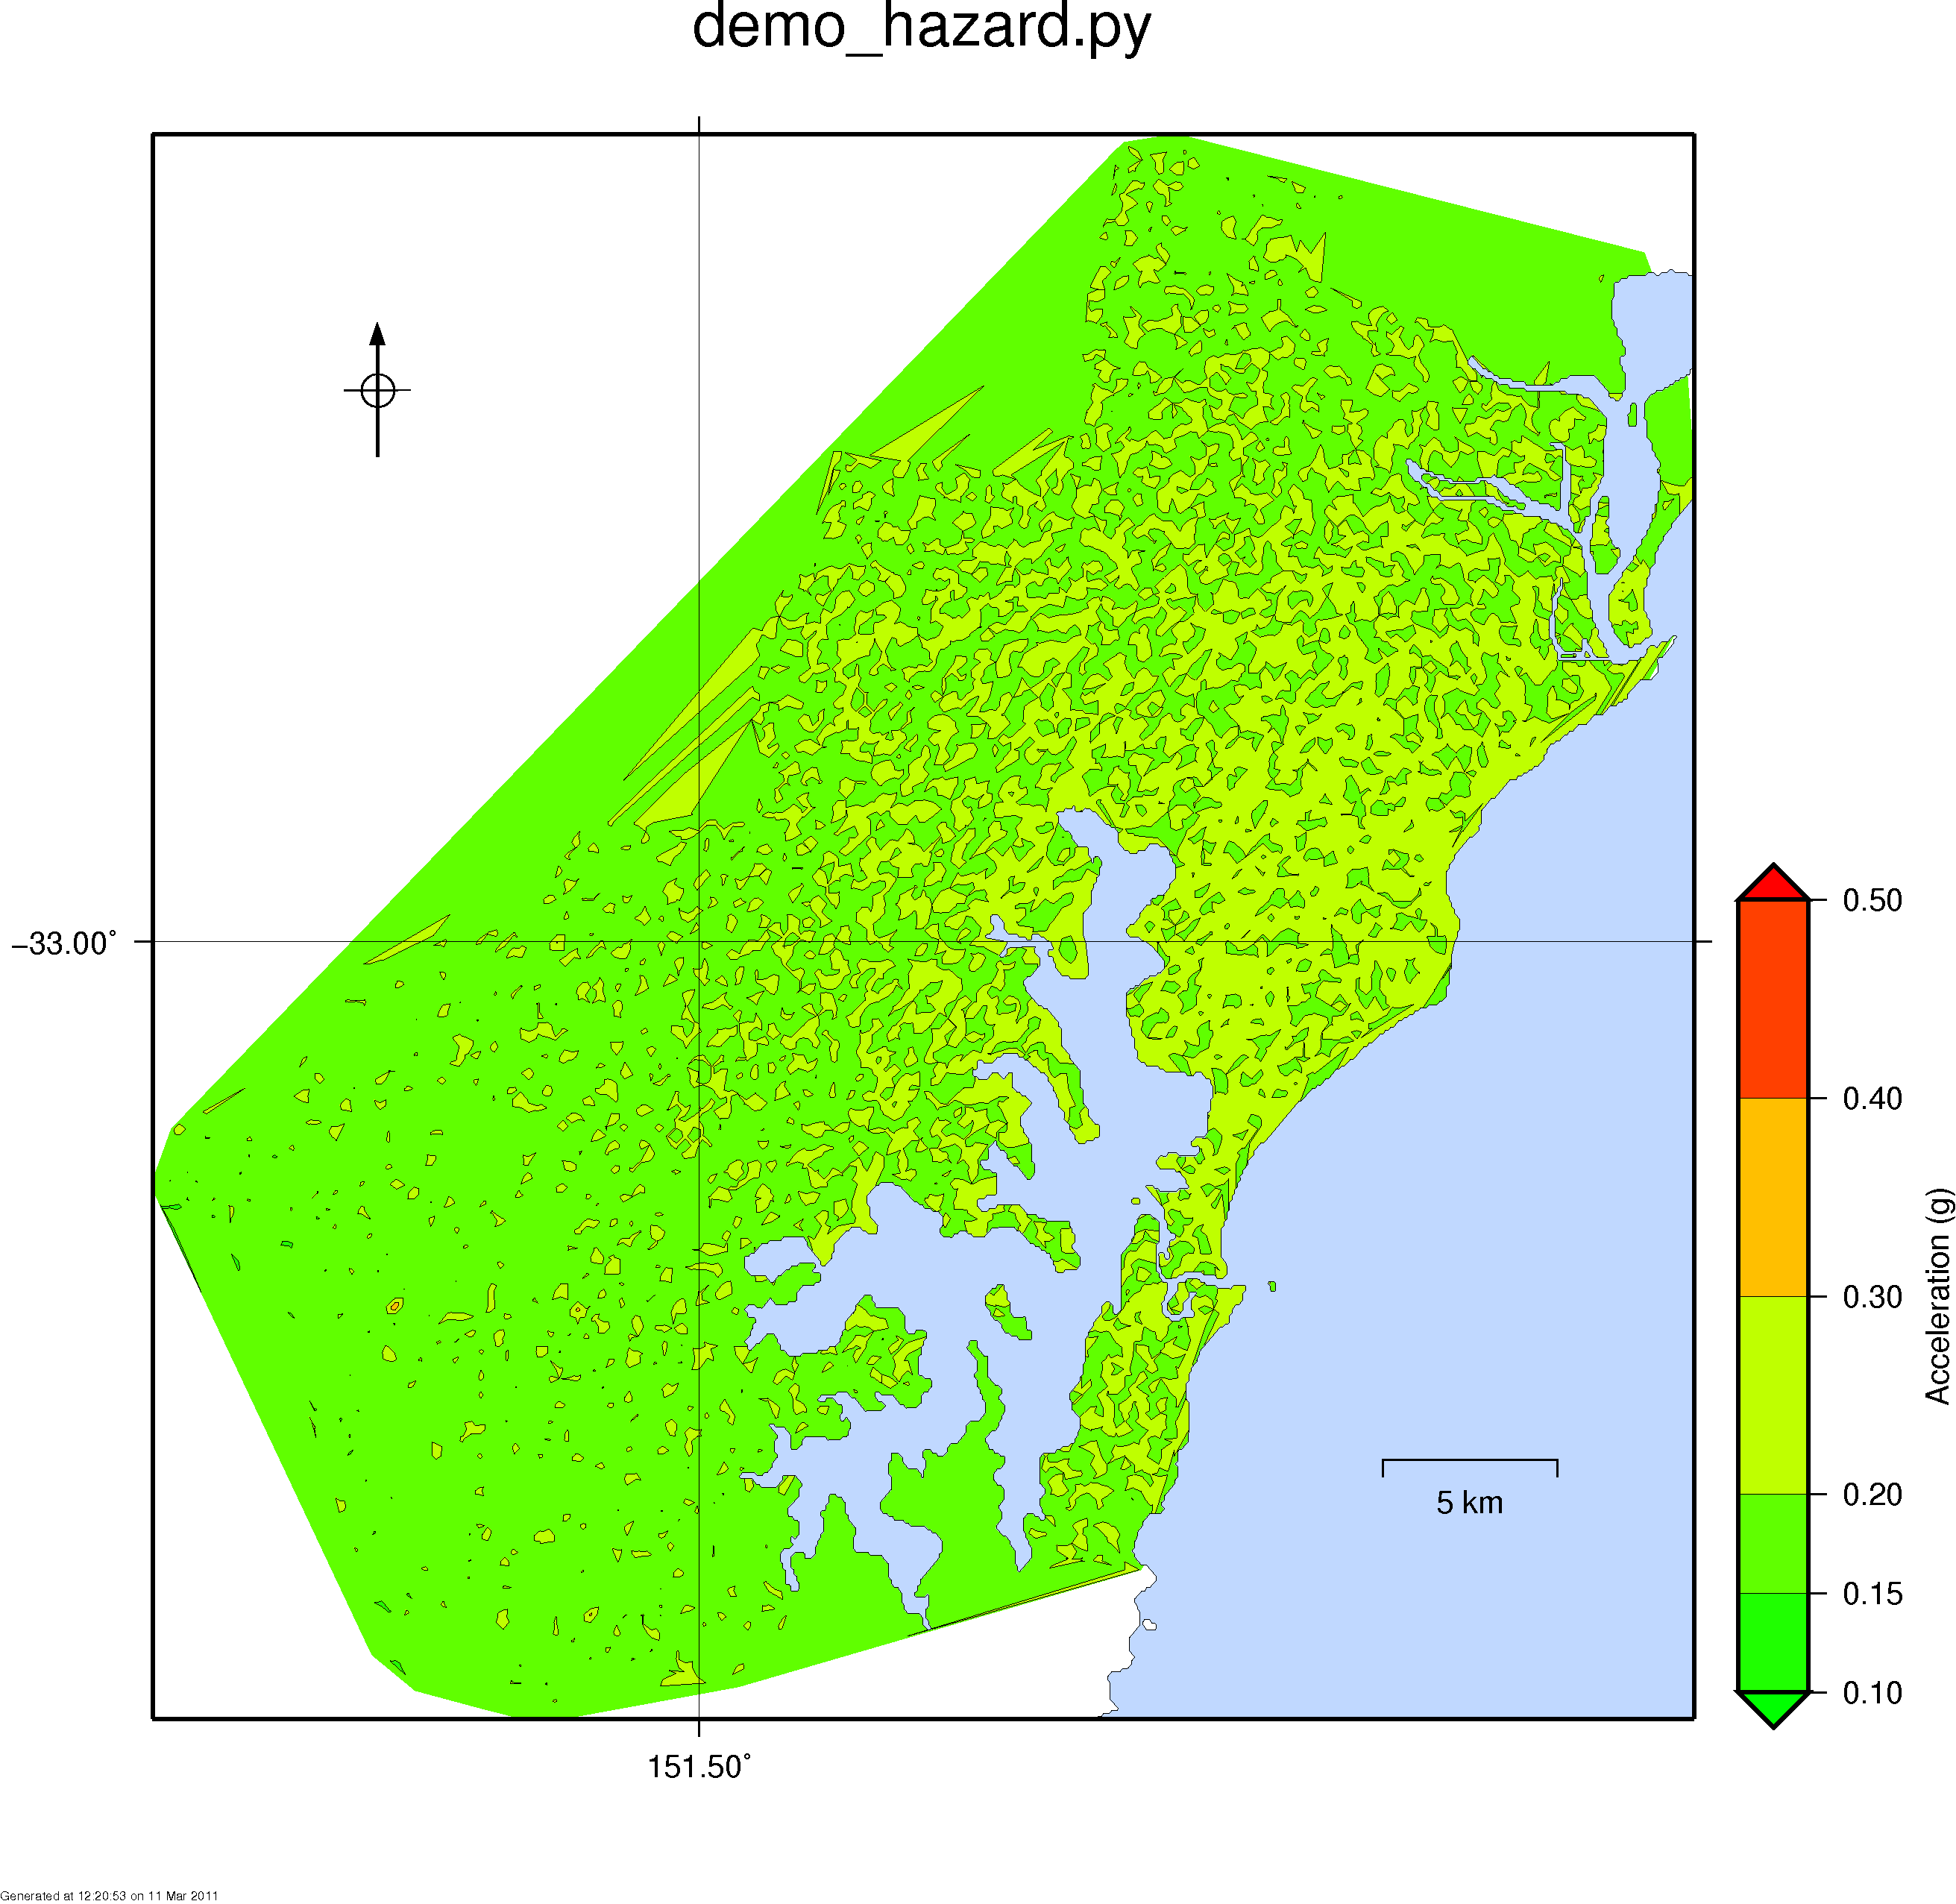
\includegraphics[width=1\textwidth]{demo_hazard}
\caption{Newcastle and Lake Macquarie hazard map for return period
of 500 years and $S_a$ period of 0.3 seconds}
\label{fig:risk-hazardmap}
\end{figure}
\fref{fig:risk-hazardmap} provides an example of a hazard map for
the Newcastle and Lake Macquarie region.

It is necessary to draw a number of hazard maps corresponding to
different $T_o$ and $R_Y$ in order to understand the hazard across
a spatial region. Traditionally return periods considered for
building design correspond to a 2\% and/or 10\% probability of
exceedance within 50 years. An exceedance probability of 10\% in
50 years equates to a return period of roughly 500 years and an
exceedance probability of 2\% in 50 years corresponds to roughly
2500 years.

The EQRM post processing tool \typefunc{plot\_api.fig\_hazard}{}{} can
be used to generate hazard maps. 

\subsection{Hazard exceedance curves}

The exceedance probability curve for hazard (also known as the
hazard exceedance curve or hazard curve) represents a technique
for visualising the earthquake hazard at a single location. The
hazard exceedance curve expresses $P(Y \ge y)$ at a single
location as a function of the earthquake hazard ($Y = S_a$). Note
that unlike the hazard map, the hazard exceedance curve presents
the hazard corresponding to the `full' range of probability levels
(return periods).
\begin{figure}
%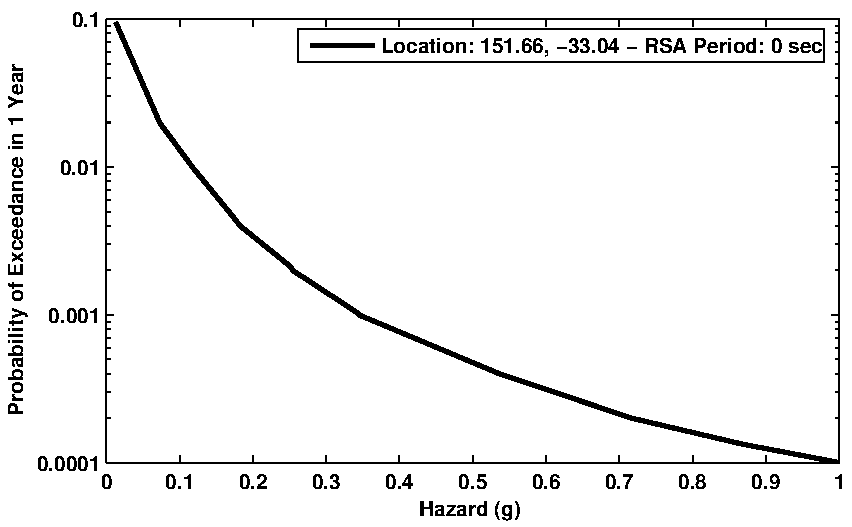
\includegraphics{fig-risk-hzdexceedcurve}
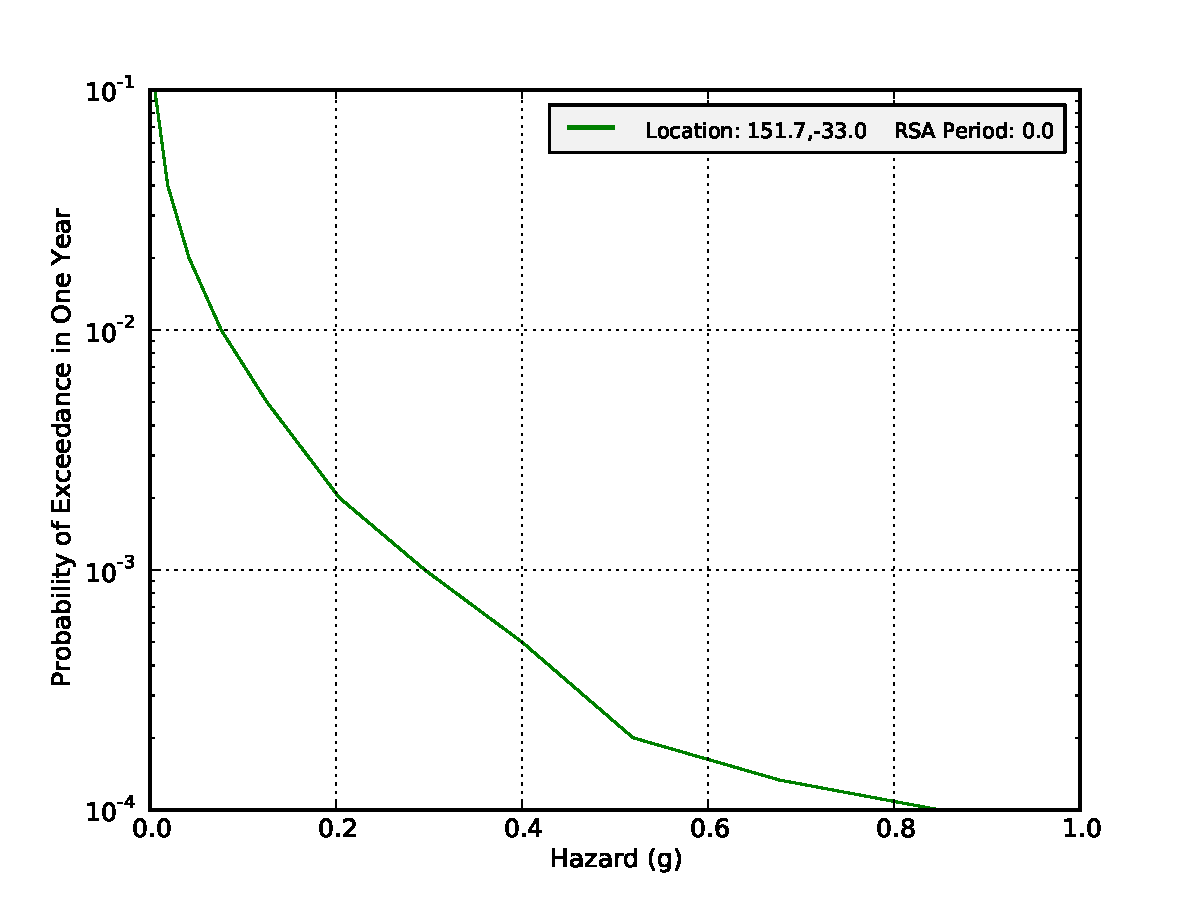
\includegraphics[width=1\textwidth]{demo_hazard_exceedance}
\caption{Peak ground acceleration hazard exceedance curve for the
Newcastle central business district.}
\label{fig:risk-hzdexceedcurve}
\end{figure}
\fref{fig:risk-hzdexceedcurve} provides an example of a hazard
exceedance curve for the Newcastle central business district. The
EQRM post processing tool \typefunc{plot\_api.fig\_hazard\_exceedance}{}{} can
be used to generate hazard exceedance curves.


\section{Earthquake risk results}

The EQRM returns the loss for each earthquake-building pair. This
information is saved in an output file along with
other information such as building values, the event activity for
each synthetic earthquake and the distance between the
building-earthquake pair. It is important to note that this
technique for data storage is fundamentally different to the
technique used for storing the earthquake hazard outputs. Recall
that the earthquake hazard outputs store only the earthquake
hazard values and not the $S_a$ at each site. Saving the
information for each earthquake-building pair provides greater
flexibility for risk visualisation and allows the de-aggregation
of risk results into a variety of forms. As a result risk output
files are typically much larger than hazard outputs and computer
memory can become problematic. When the EQRM runs out of memory in
a risk simulation the user needs to reduce the number of synthetic
earthquakes and/or the number of buildings in the building
catalogue. If reducing the number of earthquake-building pairs is
not possible the EQRM can be run in a cut-down mode that saves
risk results rather than earthquake-building pairs.

The EQRM is equipped with tools for visualising earthquake risk in
the following forms:
\begin{enumerate}
\item the risk exceedance curve (PML), \item annualised loss, and
\item a variety of disaggregated annualised loss values.
\end{enumerate}
The manner in which the output file is processed will vary slightly
depending on the plotting tool being used.  However, all of the
plotting tools make use of the basic process described by
\ereftwo{eq:eva-vectors1}{eq:eva-vectors2} where the random variable
$Y$ describes the loss.

\subsection{Risk exceedance curve}

The exceedance probability curve for risk is analogous to the
exceedance probability curve for hazard. The curve represents the
maximum loss that is expected to be exceeded for given levels of
probability. Unlike the hazard exceedance curve the risk
exceedance curve need not be presented for a single site. It is
more common to represent the percentage loss for an entire
portfolio of buildings, however risk exceedance curves for single
buildings can also be constructed. The risk exceedance curve
expresses $P(Y \ge y)$ as a function of the earthquake risk
$Y=E_L$, where $E_L$ may be the percentage loss to the portfolio
or the loss to a single building.
\begin{figure}
%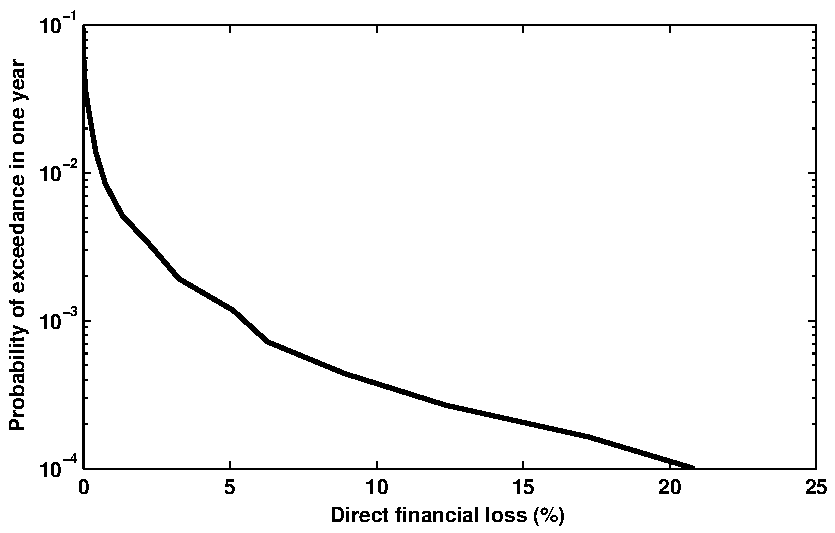
\includegraphics{fig-risk-pml}
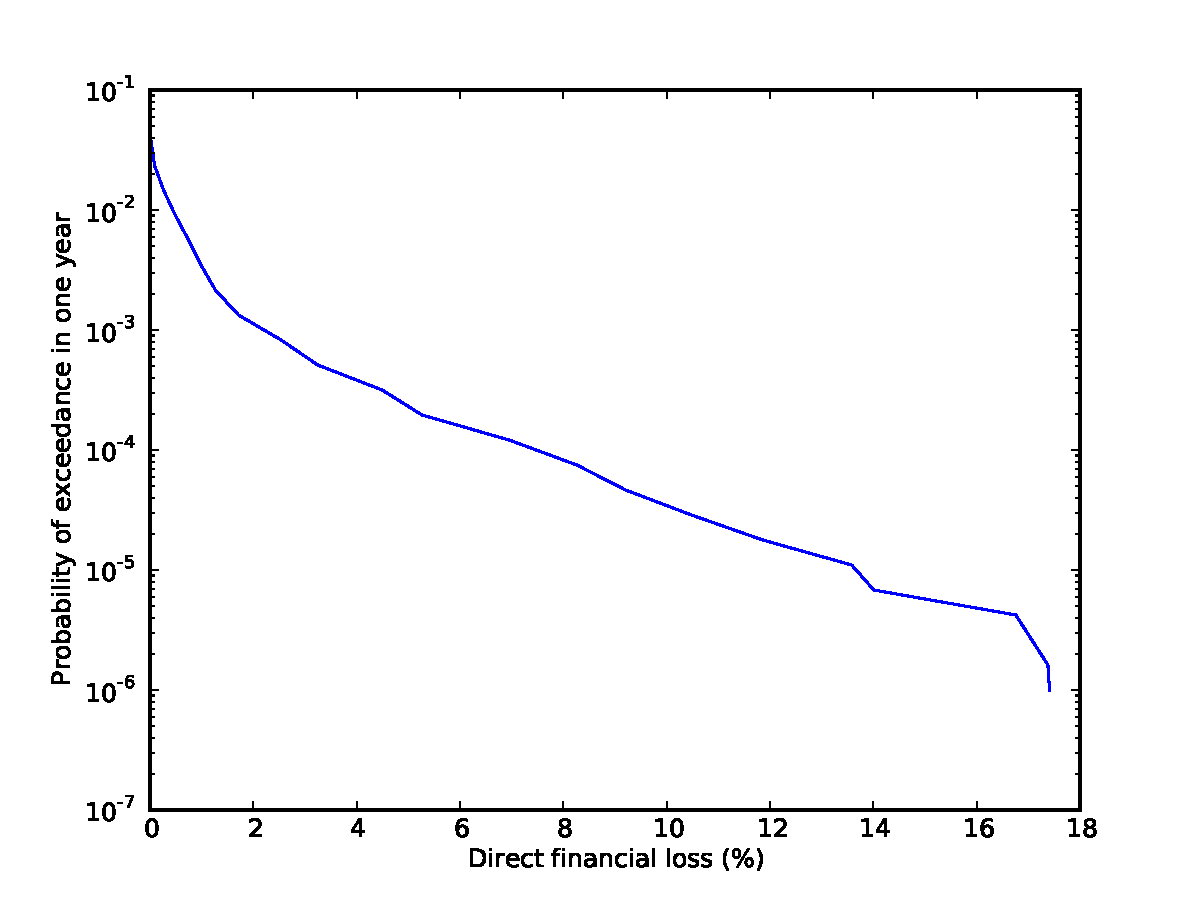
\includegraphics[width=1\textwidth]{demo_loss_exceedance}
\caption{Risk exceedance curve for all the buildings in the
Newcastle and Lake Macquarie portfolio.} \label{fig-risk-pml}
\end{figure}
\fref{fig-risk-pml} provides an example of a risk exceedance curve
for the Newcastle and Lake Macquarie portfolio.  The
EQRM post processing tool
\typefunc{plot\_api.fig\_loss\_exceedance}{}{} can be used
 to plot a
risk exceedance curve.

\subsection{Annualised loss}

The annualised loss represents the loss per year averaged over all
of the synthetic earthquakes. It can be computed by integrating
underneath the risk exceedance curve. Since this is not
necessarily intuitive the proof is given below.

Consider the risk exceedance curve as the probability of a loss
being exceeded in a one year time frame $P(Y \ge y)$. Let
$f_{E_L}(\ell)$ denote the PDF (probability density function) of
the aggregate loss and $F_{E_L}(\ell)$ denote the CDF (cumulative
distribution function). Let us define $F_{E_L}(\ell)$ as the CDF,
$$
 F_{E_L}(\ell) = \int_0^\ell f(x)\, dx.
$$
and $G(\ell)$ as the exceedence probability function,
$$
 G_{E_L}(\ell) = 1 - F_{E_L}(\ell) = \int_\ell^\infty f_{E_L}(y)\,dy.
$$
The mean of the random variable $E_L$ or annualised loss is given
by the expectation
$$
 E(L) = \int_0^\infty y f_{E_L}(y)\,dy.
$$
Using integration by parts, and using $f_{E_L}(y) =
-G'_{E_L}(\ell)$, we get
$$
 E(L) = \int_0^\infty -y G'_{E_L}(y)\,dy
      =  \big[ -yG_{E_L}(y)\big]_0^\infty + \int_0^\infty
      G_{E_L}(y)\,dy.
$$

Assuming $xG_{E_L}\to 0$ as $x\to\infty$ (which is true for an
exponential distribution, or distribution which behaves
asymptotically as exponential) we have
$$
 E(L) = \int_0^\infty G_{E_L}(y)\,dy
$$
which demonstrates that the mean value of the loss is the area
under the risk exceedance curve (PML).


\subsection{Disaggregated annualised loss}

Storing the loss results for all of the earthquake-building pairs
allows the de-aggregation of annualised loss into a couple of
classes. The EQRM offers several tools to assist the
de-aggregation into common classes. These
are described as follows:
\begin{figure}
%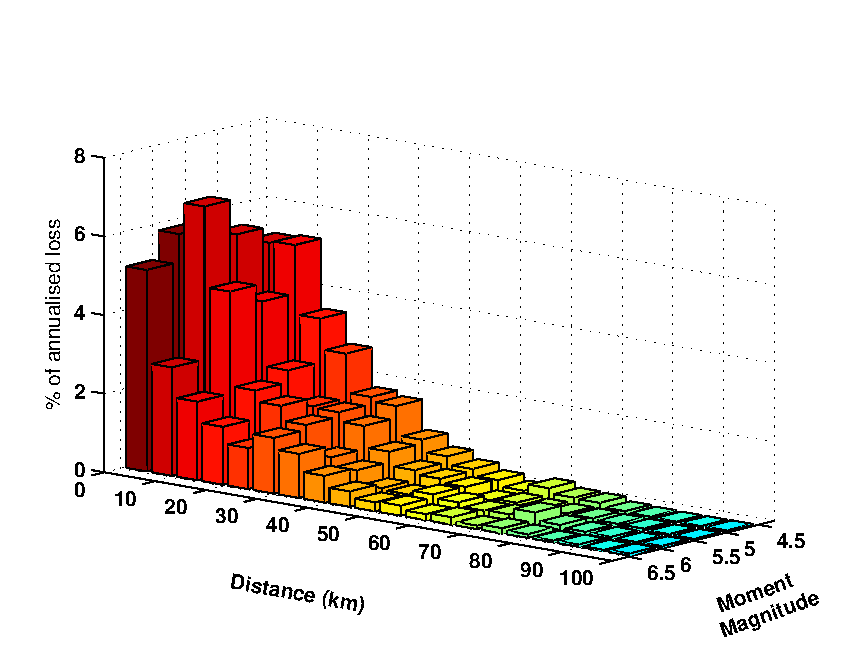
\includegraphics{fig-risk-deaggdistmag}
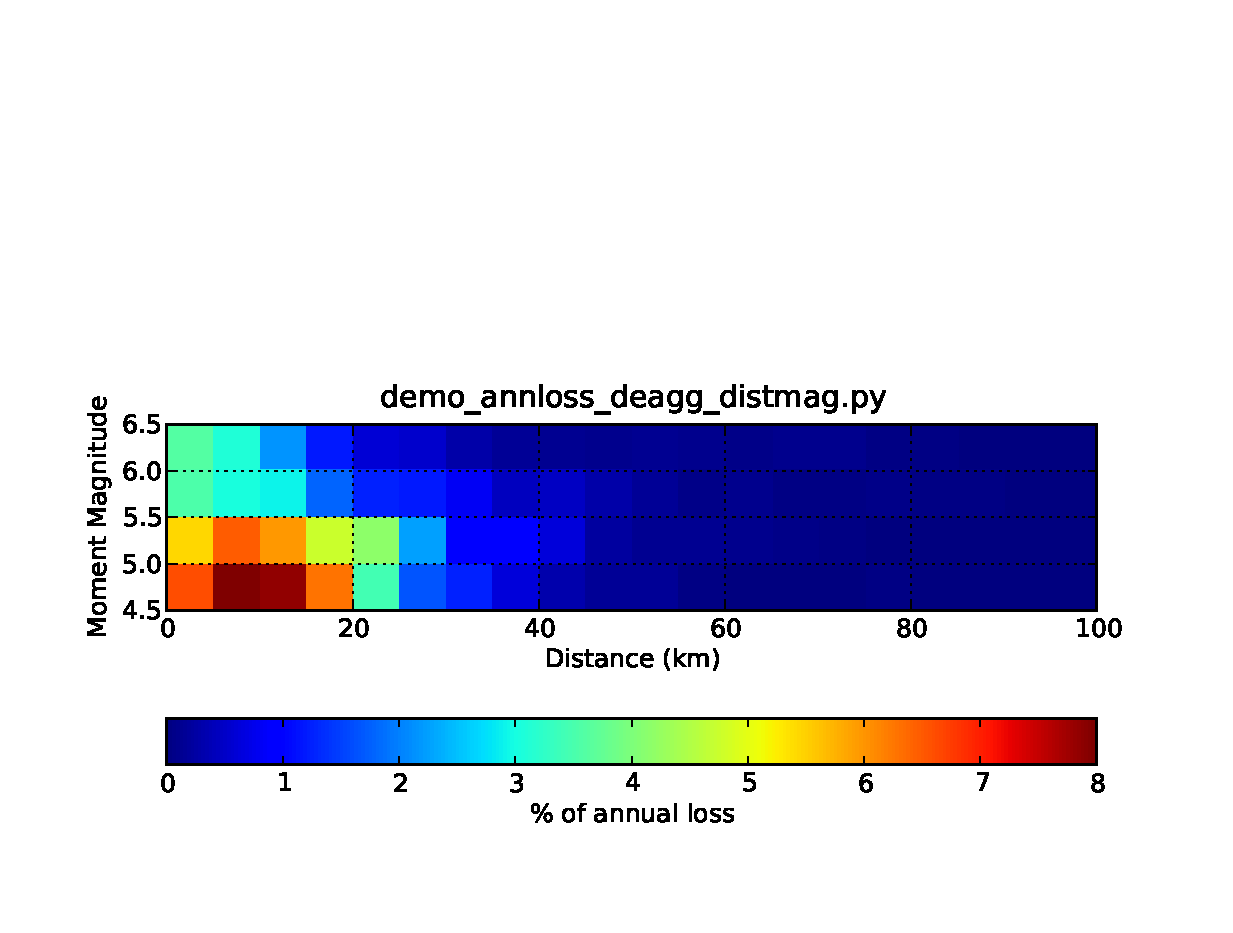
\includegraphics[width=1\textwidth]{demo_annloss_deagg_distmag}
 \caption{Annualised loss
disaggregated by distance and magnitude for the Newcastle and Lake
Macquarie region.} \label{fig-risk-deaggdistmag}
\end{figure}

\begin{enumerate}
\item \textbf{disaggregation by distance and magnitude} allows the
visualisation of magnitude-distance combinations which have the
greatest influence on risk assessments.
\fref{fig-risk-deaggdistmag} illustrates the disaggregation by
distance and magnitude for risk in the Newcastle and Lake
Macquarie region. The individual plotting tool
\typefunc{plot\_api.fig\_annloss\_deagg\_distmag}{}{} can be used
to de-aggregate the risk by
distance and magnitude. 

\item \textbf{disaggregation by cells} separates
the annualised loss into different cells and allows the
visualisation of how earthquake risk varies spatially. The
individual plotting tool
\typefunc{plot\_api.fig\_annloss\_deagg\_cells}{}{} can be used 
 to de-aggregate the risk by
cells. 
\end{enumerate}

\section{Earthquake scenario results}

The output for an earthquake scenario loss simulation is 
stored in the file
\typepar{<output\_dir>} directory. 
\begin{figure}
%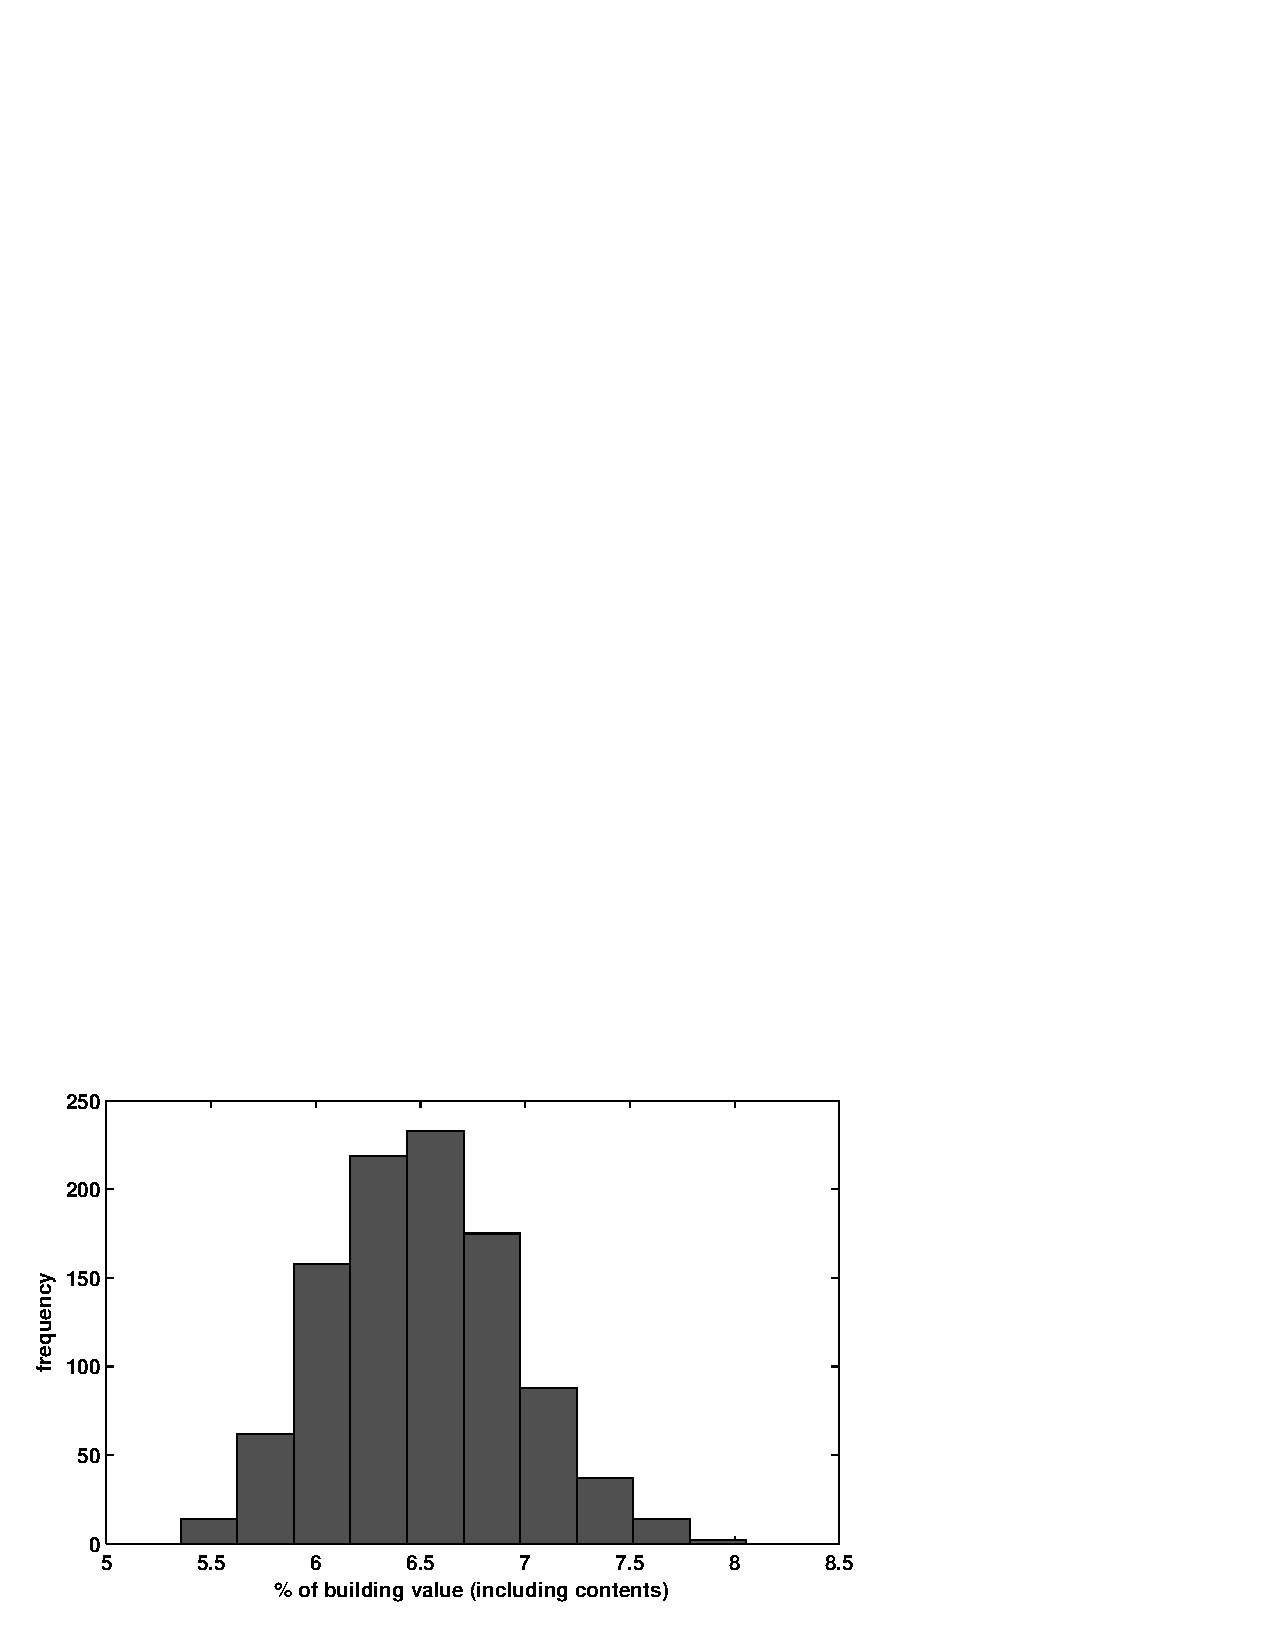
\includegraphics{fig-risk-scen-hist}
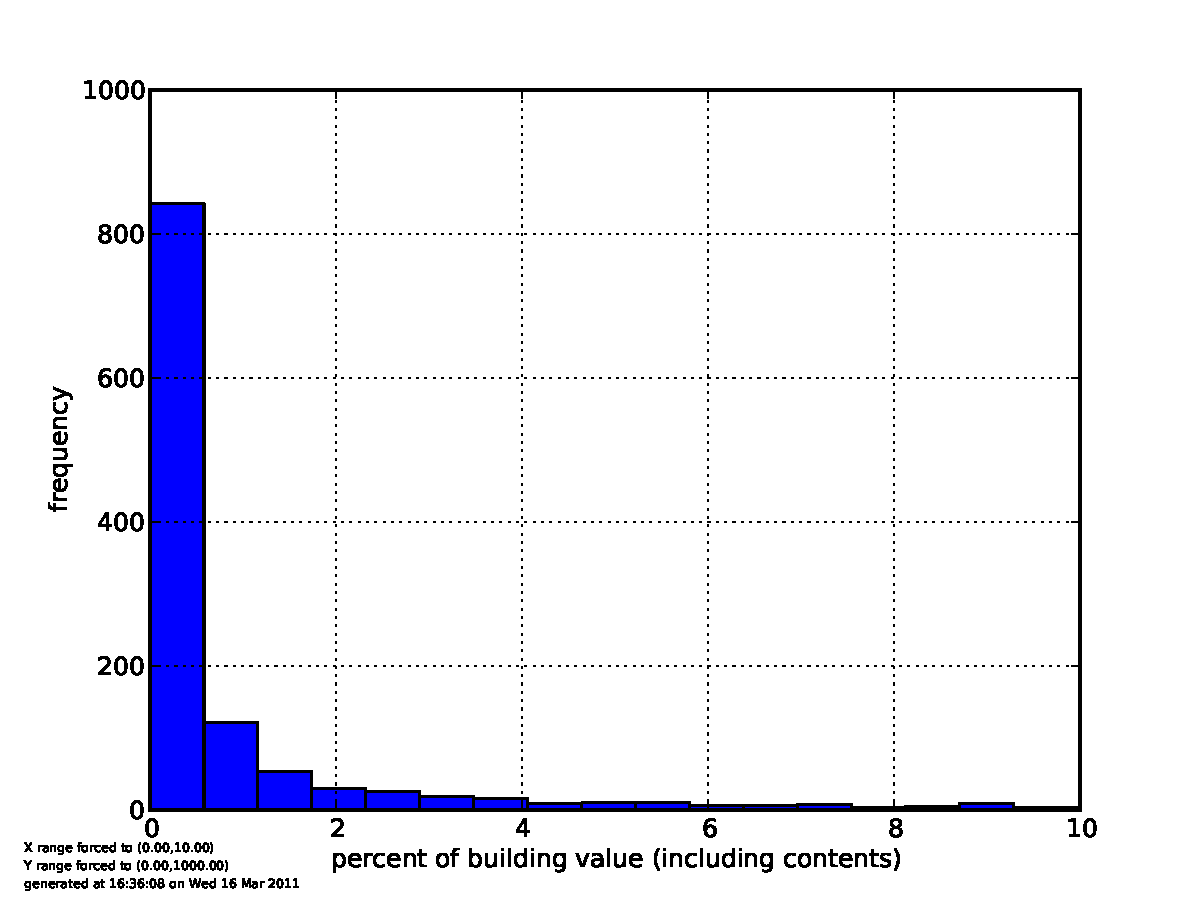
\includegraphics[width=1\textwidth]{demo_scenario_building_loss_percent}
\caption{Histogram of loss estimates for a synthetic Newcastle
1989 earthquake.} \label{fig:scenario-hist}
\end{figure}
The primary technique for visualising an EQRM scenario output is
via a histogram such as that shown in \fref{fig:scenario-hist} for
a simulation of the Newcastle 1989 earthquake. Each bar of the
histogram in \fref{fig:scenario-hist} represents the frequency of
realisations which predicted a loss value within the bars domain.
Histograms such as \fref{fig:scenario-hist} can be produced using
the individual plotting tool
\typefunc{plot\_api.fig\_scenario\_building\_loss\_percentage}{}{}.


